Part of speech tagging is probably one the most common NLP tasks. The
task is to assign each word with a grammatical category, i.e Noun,
Verb, Adjective, ... . In English, using the Penn Treebank (ptb)~\citep{pennTreeBank} the current
state of the art for part of speech tagging is around the 97\% for a
variety of methods \footnote{See ACL state of the art wiki}.

In the rest of this class we will use a subset of the ptb corpus, but
instead of using the original 45 tags we will use a reduced tag set of
12 tags, to make the algorithms faster for the
class. In this task, $\sent$ is a sentence and $\hseq$
is the sequence of possible PoS tags.

The first step is to load the pos corpus, we will start by loading
1000 sentences for training and 200 sentences both for development and
testing, and train the HMM model.
\begin{python}
In []: run readers/pos_corpus.py
In []: posc = PostagCorpus("en",max_sent_len=15,train_sents=1000,dev_sents=200,test_sents=200)
In []: run sequences/hmm.py
In []: hmm = HMM(posc)
In []: hmm.train_supervised(posc.train)
Warning: invalid value encountered in divide
\end{python}

Note the warning ``Warning: invalid value encountered in divide``
again due to the lack of smoothing. This is because we are trying to
estimate the probability of words that were never seen during
training, so the counts are zero and we are trying to do 0/0. 

Look at the transitions probabilities of the trained model (see
Figure \ref{fig:transProbs}) and see if they match your intuition
about the English language (e.g. adjectives tend to come before nouns).

\begin{figure}
\centering
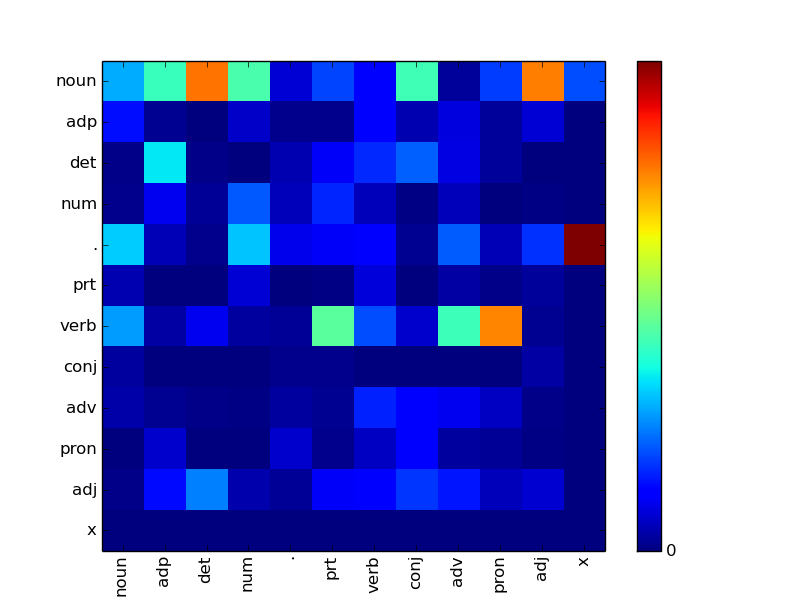
\includegraphics[scale=.5]{figs/sequences/transition_probs}
\caption{\label{fig:transProbs} Transition probabilities of the
trained model. Each column is previous state and row is current
state. Note the high probability of having Noun after Adjective, as expected.}
\end{figure}

\begin{exercise}
Test the model using both posterior decoding and viterbi decoding on
both the train and test set, using the methods in class HMM:
\begin{python}
viterbi_decode_corpus(self,seq_list)
posterior_decode_corpus(self,seq_list)
evaluate_corpus(self,seq_list,predictions)
\end{python}

What do you observe. Remake the previous exercise but now train the HMM
using smoothing. Try different values and report the results on the
train and development set (1,0.1,0.001,0.0001). (Use function
\emph{pick\_best\_smoothing}).


\begin{python}
In []: hmm.pick_best_smoothing(posc.train,posc.dev,[0,0.1,0.01,1])
Warning: invalid value encountered in divide
Smoothing 0.000000 --  Train Set Accuracy: Posterior Decode 0.985, Viterbi Decode: 0.985
Smoothing 0.000000 -- Test Set Accuracy: Posterior Decode 0.177, Viterbi Decode: 0.381
Smoothing 0.100000 --  Train Set Accuracy: Posterior Decode 0.971, Viterbi Decode: 0.967
Smoothing 0.100000 -- Test Set Accuracy: Posterior Decode 0.852, Viterbi Decode: 0.836
Smoothing 0.010000 --  Train Set Accuracy: Posterior Decode 0.983, Viterbi Decode: 0.982
Smoothing 0.010000 -- Test Set Accuracy: Posterior Decode 0.816, Viterbi Decode: 0.809
Smoothing 1.000000 --  Train Set Accuracy: Posterior Decode 0.890, Viterbi Decode: 0.876
Smoothing 1.000000 -- Test Set Accuracy: Posterior Decode 0.857, Viterbi Decode: 0.829
\end{python}

Using the best smoothing value evaluate the accuracy on the test set.

\begin{python}
In []: run readers/pos_corpus.py
In []: posc = PostagCorpus("en",max_sent_len=15,train_sents=1000,dev_sents=200,test_sents=200)
In []: run sequences/hmm.py
In []: hmm = HMM(posc)
In []: hmm.train_supervised(posc.train,smoothing=1)
In []: pred = hmm.viterbi_decode_corpus(posc.test.seq_list)
In []: eval_test = hmm.evaluate_corpus(posc.test.seq_list,pred)
In []: eval_test
Out[]: 0.77711397058823528
\end{python}

Perform some error analysis to understand were the errors are coming
from. You can start visualizing the confusion matrix (true tags vs
predicted tags).

\begin{python}
In []: run sequences/confusion_matrix.py
In []: cm = build_confusion_matrix(posc.test.seq_list,pred,len(posc.int_to_pos),hmm.nr_states)
\end{python}

\begin{figure}
\centering
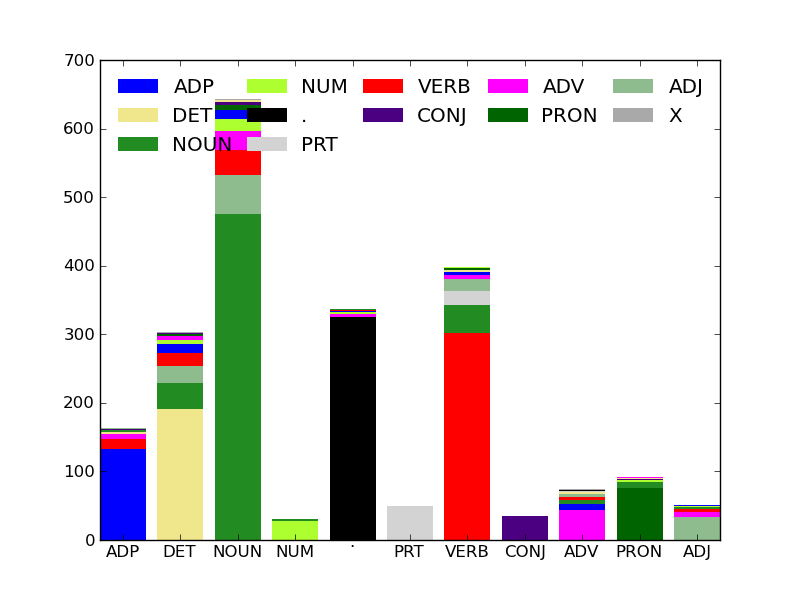
\includegraphics[scale=.5]{figs/sequences/cm_sup.png}
\caption{\label{fig:cm_uns} Confusion Matrix for the previous
  example. Predict tags are columns and the true tags corresponds to
  the constituents of each column.}
\end{figure}

Another option to look at is to the error for words with different
number of occurrences, rare words vs commons words.
\end{exercise}


\begin{exercise}
Implement a function that produces the accuracy for rare words vs
common words. Use you own definition of rare word.

Can you come up with other error analysis methods? Which?

\end{exercise}

\begin{exercise}
So far we have only worked with a limited dataset of 1000 words. In
this exercise you will test the accuracy of the HMM model for
different training sizes (1000,5000,10000,50000). What do you observe?

\end{exercise}
